\PassOptionsToPackage{unicode=true}{hyperref} % options for packages loaded elsewhere
\PassOptionsToPackage{hyphens}{url}
%
\documentclass[]{article}
\usepackage{lmodern}
\usepackage{amssymb,amsmath}
\usepackage{ifxetex,ifluatex}
\usepackage{fixltx2e} % provides \textsubscript
\ifnum 0\ifxetex 1\fi\ifluatex 1\fi=0 % if pdftex
  \usepackage[T1]{fontenc}
  \usepackage[utf8]{inputenc}
  \usepackage{textcomp} % provides euro and other symbols
\else % if luatex or xelatex
  \usepackage{unicode-math}
  \defaultfontfeatures{Ligatures=TeX,Scale=MatchLowercase}
\fi
% use upquote if available, for straight quotes in verbatim environments
\IfFileExists{upquote.sty}{\usepackage{upquote}}{}
% use microtype if available
\IfFileExists{microtype.sty}{%
\usepackage[]{microtype}
\UseMicrotypeSet[protrusion]{basicmath} % disable protrusion for tt fonts
}{}
\IfFileExists{parskip.sty}{%
\usepackage{parskip}
}{% else
\setlength{\parindent}{0pt}
\setlength{\parskip}{6pt plus 2pt minus 1pt}
}
\usepackage{hyperref}
\hypersetup{
            pdftitle={Stochastische Ausarbeitung},
            pdfauthor={Bela},
            pdfborder={0 0 0},
            breaklinks=true}
\urlstyle{same}  % don't use monospace font for urls
\usepackage[margin=1in]{geometry}
\usepackage{color}
\usepackage{fancyvrb}
\newcommand{\VerbBar}{|}
\newcommand{\VERB}{\Verb[commandchars=\\\{\}]}
\DefineVerbatimEnvironment{Highlighting}{Verbatim}{commandchars=\\\{\}}
% Add ',fontsize=\small' for more characters per line
\usepackage{framed}
\definecolor{shadecolor}{RGB}{248,248,248}
\newenvironment{Shaded}{\begin{snugshade}}{\end{snugshade}}
\newcommand{\AlertTok}[1]{\textcolor[rgb]{0.94,0.16,0.16}{#1}}
\newcommand{\AnnotationTok}[1]{\textcolor[rgb]{0.56,0.35,0.01}{\textbf{\textit{#1}}}}
\newcommand{\AttributeTok}[1]{\textcolor[rgb]{0.77,0.63,0.00}{#1}}
\newcommand{\BaseNTok}[1]{\textcolor[rgb]{0.00,0.00,0.81}{#1}}
\newcommand{\BuiltInTok}[1]{#1}
\newcommand{\CharTok}[1]{\textcolor[rgb]{0.31,0.60,0.02}{#1}}
\newcommand{\CommentTok}[1]{\textcolor[rgb]{0.56,0.35,0.01}{\textit{#1}}}
\newcommand{\CommentVarTok}[1]{\textcolor[rgb]{0.56,0.35,0.01}{\textbf{\textit{#1}}}}
\newcommand{\ConstantTok}[1]{\textcolor[rgb]{0.00,0.00,0.00}{#1}}
\newcommand{\ControlFlowTok}[1]{\textcolor[rgb]{0.13,0.29,0.53}{\textbf{#1}}}
\newcommand{\DataTypeTok}[1]{\textcolor[rgb]{0.13,0.29,0.53}{#1}}
\newcommand{\DecValTok}[1]{\textcolor[rgb]{0.00,0.00,0.81}{#1}}
\newcommand{\DocumentationTok}[1]{\textcolor[rgb]{0.56,0.35,0.01}{\textbf{\textit{#1}}}}
\newcommand{\ErrorTok}[1]{\textcolor[rgb]{0.64,0.00,0.00}{\textbf{#1}}}
\newcommand{\ExtensionTok}[1]{#1}
\newcommand{\FloatTok}[1]{\textcolor[rgb]{0.00,0.00,0.81}{#1}}
\newcommand{\FunctionTok}[1]{\textcolor[rgb]{0.00,0.00,0.00}{#1}}
\newcommand{\ImportTok}[1]{#1}
\newcommand{\InformationTok}[1]{\textcolor[rgb]{0.56,0.35,0.01}{\textbf{\textit{#1}}}}
\newcommand{\KeywordTok}[1]{\textcolor[rgb]{0.13,0.29,0.53}{\textbf{#1}}}
\newcommand{\NormalTok}[1]{#1}
\newcommand{\OperatorTok}[1]{\textcolor[rgb]{0.81,0.36,0.00}{\textbf{#1}}}
\newcommand{\OtherTok}[1]{\textcolor[rgb]{0.56,0.35,0.01}{#1}}
\newcommand{\PreprocessorTok}[1]{\textcolor[rgb]{0.56,0.35,0.01}{\textit{#1}}}
\newcommand{\RegionMarkerTok}[1]{#1}
\newcommand{\SpecialCharTok}[1]{\textcolor[rgb]{0.00,0.00,0.00}{#1}}
\newcommand{\SpecialStringTok}[1]{\textcolor[rgb]{0.31,0.60,0.02}{#1}}
\newcommand{\StringTok}[1]{\textcolor[rgb]{0.31,0.60,0.02}{#1}}
\newcommand{\VariableTok}[1]{\textcolor[rgb]{0.00,0.00,0.00}{#1}}
\newcommand{\VerbatimStringTok}[1]{\textcolor[rgb]{0.31,0.60,0.02}{#1}}
\newcommand{\WarningTok}[1]{\textcolor[rgb]{0.56,0.35,0.01}{\textbf{\textit{#1}}}}
\usepackage{longtable,booktabs}
% Fix footnotes in tables (requires footnote package)
\IfFileExists{footnote.sty}{\usepackage{footnote}\makesavenoteenv{longtable}}{}
\usepackage{graphicx,grffile}
\makeatletter
\def\maxwidth{\ifdim\Gin@nat@width>\linewidth\linewidth\else\Gin@nat@width\fi}
\def\maxheight{\ifdim\Gin@nat@height>\textheight\textheight\else\Gin@nat@height\fi}
\makeatother
% Scale images if necessary, so that they will not overflow the page
% margins by default, and it is still possible to overwrite the defaults
% using explicit options in \includegraphics[width, height, ...]{}
\setkeys{Gin}{width=\maxwidth,height=\maxheight,keepaspectratio}
\setlength{\emergencystretch}{3em}  % prevent overfull lines
\providecommand{\tightlist}{%
  \setlength{\itemsep}{0pt}\setlength{\parskip}{0pt}}
\setcounter{secnumdepth}{5}
% Redefines (sub)paragraphs to behave more like sections
\ifx\paragraph\undefined\else
\let\oldparagraph\paragraph
\renewcommand{\paragraph}[1]{\oldparagraph{#1}\mbox{}}
\fi
\ifx\subparagraph\undefined\else
\let\oldsubparagraph\subparagraph
\renewcommand{\subparagraph}[1]{\oldsubparagraph{#1}\mbox{}}
\fi

% set default figure placement to htbp
\makeatletter
\def\fps@figure{htbp}
\makeatother


\title{Stochastische Ausarbeitung}
\author{Bela}
\date{10.04.2023}

\begin{document}
\maketitle

{
\setcounter{tocdepth}{2}
\tableofcontents
}
\hypertarget{einleitung}{%
\section{Einleitung}\label{einleitung}}

Viel Spaß mit meiner Ausarbeitung :).

\hypertarget{aufagabe-1}{%
\section{Aufagabe 1}\label{aufagabe-1}}

\hypertarget{chi2-anpassungstest}{%
\subsection{\texorpdfstring{\(\chi^2\)-Anpassungstest}{\textbackslash{}chi\^{}2-Anpassungstest}}\label{chi2-anpassungstest}}

In der Multinomialverteilung haben wir \(4\) Kategorien, welche jeweils Binomial verteilt sind.
Für große \(n\) ist die Binomialverteilung normalverteilt mit \(\mu = n \cdot p\) und \(\sigma = \sqrt{n \cdot p \cdot (1-p)}\).
Sei \(a_1, a_2, a_3, a_4\) die Anzahl der Beobachtungen in den Kategorien. Damit ist \(\dfrac{a_j-n \cdot p_j}{\sqrt{n \cdot p_j \cdot (1-p_j)}}\sim N(0,1)\).
Also ist \(\dfrac{(a_j-n \cdot p_j)^2}{n \cdot p_j \cdot (1-p_j)}\sim (N(0,1))^2\)\\
Damit ist die Summe \(\sum_{j=1}^4 \dfrac{(a_j-n \cdot p_j)^2}{n \cdot p_j \cdot (1-p_j)}\sim \chi^2_3\).\\
Da die p-Werte der \(\chi^2\)-Verteilung bekannt sind, kann so ein einfacher Hypothesentest durchgeführt werden:

\[\begin{aligned}H_0: p_1 = \frac18, p_2 = \frac14, p_3 = \frac12, p_4 = \frac18  \\
H_1: Nicht alle p_j haben werte wie H_0\end{aligned}\]

Simulieren wir nun den Versuch:

\begin{Shaded}
\begin{Highlighting}[]
\KeywordTok{set.seed}\NormalTok{(}\DecValTok{123}\NormalTok{)}
\NormalTok{simulateAnpassungstest <-}\StringTok{ }\ControlFlowTok{function}\NormalTok{()\{}
\NormalTok{  n <-}\StringTok{ }\DecValTok{1000}
\NormalTok{  p <-}\StringTok{ }\KeywordTok{c}\NormalTok{(}\DecValTok{1}\OperatorTok{/}\DecValTok{8}\NormalTok{, }\DecValTok{1}\OperatorTok{/}\DecValTok{4}\NormalTok{, }\DecValTok{1}\OperatorTok{/}\DecValTok{2}\NormalTok{, }\DecValTok{1}\OperatorTok{/}\DecValTok{8}\NormalTok{)}
\NormalTok{  a <-}\StringTok{ }\KeywordTok{rmultinom}\NormalTok{(}\DecValTok{1}\NormalTok{, n, p)}
  \KeywordTok{sum}\NormalTok{((a }\OperatorTok{-}\StringTok{ }\NormalTok{n}\OperatorTok{*}\NormalTok{p)}\OperatorTok{^}\DecValTok{2}\OperatorTok{/}\NormalTok{(n}\OperatorTok{*}\NormalTok{p))}
\NormalTok{\}}
\end{Highlighting}
\end{Shaded}

\begin{Shaded}
\begin{Highlighting}[]
\NormalTok{results <-}\StringTok{ }\KeywordTok{c}\NormalTok{()}
\ControlFlowTok{for}\NormalTok{ (i }\ControlFlowTok{in} \DecValTok{1}\OperatorTok{:}\DecValTok{300}\NormalTok{)\{}
\NormalTok{  results =}\KeywordTok{c}\NormalTok{(results ,}\KeywordTok{simulateAnpassungstest}\NormalTok{())}
\NormalTok{\}}
\end{Highlighting}
\end{Shaded}

\begin{Shaded}
\begin{Highlighting}[]
\KeywordTok{hist}\NormalTok{(results, }\DataTypeTok{freq=}\OtherTok{FALSE}\NormalTok{, }\DataTypeTok{main =} \StringTok{"Histogramm der Chi2 Werte"}\NormalTok{, }\DataTypeTok{xlab =} \StringTok{"Chi2-Wert"}\NormalTok{, }\DataTypeTok{ylab =} \StringTok{"relative Häufigkeit"}\NormalTok{)}
\KeywordTok{curve}\NormalTok{(}\KeywordTok{dchisq}\NormalTok{(x, }\DecValTok{3}\NormalTok{), }\DataTypeTok{add =} \OtherTok{TRUE}\NormalTok{, }\DataTypeTok{col =} \StringTok{"red"}\NormalTok{)}
\end{Highlighting}
\end{Shaded}

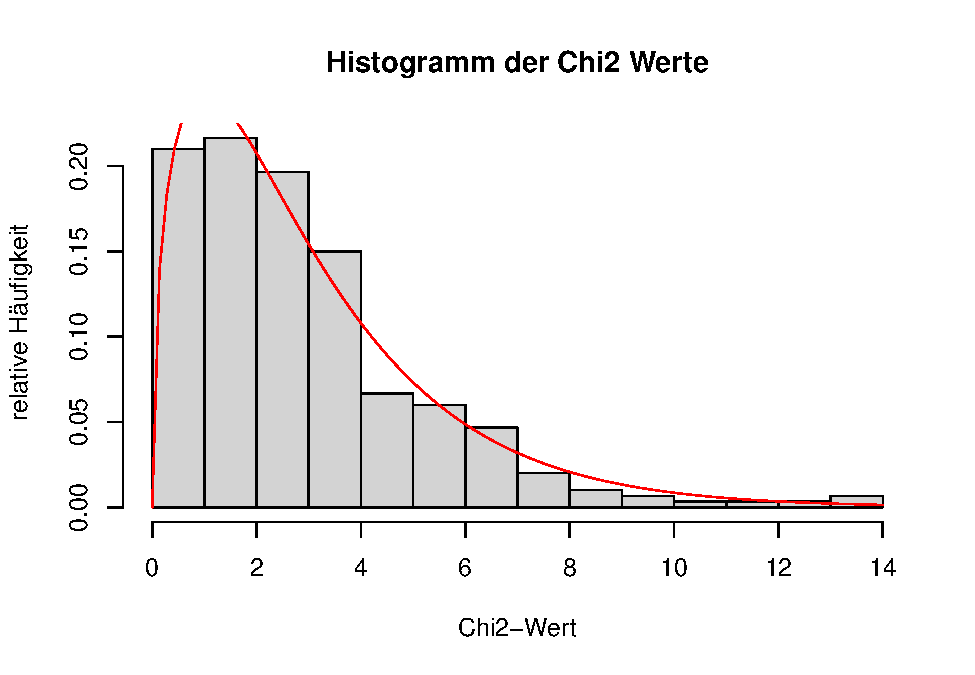
\includegraphics{Test_files/figure-latex/unnamed-chunk-3-1.pdf}

\hypertarget{t-test-mit-unbekannter-varianz}{%
\subsection{\texorpdfstring{\(t-\)Test mit unbekannter Varianz}{t-Test mit unbekannter Varianz}}\label{t-test-mit-unbekannter-varianz}}

Beim zweiseitigen \(t-\)Test mit unbekannter Varianz wird die Nullhypothese \(H_0: \mu = \mu_0\) gegen die Alternative \(H_1: \mu \neq \mu_0\) getestet.
Als Teststatistik wird \(\dfrac{\sqrt{n}(\bar X_n-\mu_0)}{S_n}\) verwendet.\\
Herleitung:\\
Seien \(X_1, X_2, \dots, X_n\sim N(\mu, \sigma^2)\) unabhängig und identisch verteilt.\\
Das arithmetische Mittel \(\bar X_n\) ist normalverteilt mit \(\mu = \mu\) und \(\sigma = \dfrac{\sigma}{\sqrt{n}}\).\\
Bei bekannter Varianz wäre \(\sqrt{n}\dfrac{\bar X_n-\mu_0}{\sigma}\sim N(0,1)\).
Wir müssen allerdings die Varianz mit der empirischen Varianz ersetzen, also ist \(\sqrt{n}\dfrac{\bar X_n-\mu_0}{S_n}\sim t_{n-1}\).(T-Verteilung folgt aus Störung durch die Varianzschätzung)

Das heißt für den Test müssen wir nur die Teststatistik \(T=\dfrac{\sqrt{n}(\bar X_n-\mu_0)}{S_n}\) berechnen und anschließend deren \(p\)-Wert bestimmen:

Test:

\begin{Shaded}
\begin{Highlighting}[]
\KeywordTok{set.seed}\NormalTok{(}\DecValTok{123}\NormalTok{)}
\NormalTok{mu0 <-}\StringTok{ }\DecValTok{2}
\NormalTok{sigma <-}\StringTok{ }\DecValTok{4}
\NormalTok{data <-}\StringTok{ }\KeywordTok{rnorm}\NormalTok{(}\DecValTok{1000}\NormalTok{, mu0, sigma)}
\NormalTok{alpha <-}\StringTok{ }\FloatTok{0.05}

\NormalTok{dataVar <-}\StringTok{ }\KeywordTok{var}\NormalTok{(data)}
\NormalTok{dataMean <-}\StringTok{ }\KeywordTok{mean}\NormalTok{(data)}

\NormalTok{T <-}\StringTok{ }\KeywordTok{sqrt}\NormalTok{(}\KeywordTok{length}\NormalTok{(data))}\OperatorTok{*}\NormalTok{(dataMean}\OperatorTok{-}\NormalTok{mu0)}\OperatorTok{/}\KeywordTok{sqrt}\NormalTok{(dataVar)}

\CommentTok{#Teststatistik}
\KeywordTok{print}\NormalTok{(}\KeywordTok{paste}\NormalTok{(}\StringTok{"T = "}\NormalTok{, T))}
\end{Highlighting}
\end{Shaded}

\begin{verbatim}
## [1] "T =  0.514279000759497"
\end{verbatim}

\begin{Shaded}
\begin{Highlighting}[]
\CommentTok{#p-Wert von T}
\KeywordTok{print}\NormalTok{(}\KeywordTok{paste}\NormalTok{(}\StringTok{"p-Wert von T = "}\NormalTok{, }\KeywordTok{pt}\NormalTok{(T, }\KeywordTok{length}\NormalTok{(data)}\OperatorTok{-}\DecValTok{1}\NormalTok{, }\DataTypeTok{lower.tail =} \OtherTok{FALSE}\NormalTok{)))}
\end{Highlighting}
\end{Shaded}

\begin{verbatim}
## [1] "p-Wert von T =  0.303585342303021"
\end{verbatim}

\begin{Shaded}
\begin{Highlighting}[]
\CommentTok{#Testresultat}
\ControlFlowTok{if}\NormalTok{ (}\KeywordTok{pt}\NormalTok{(T, }\KeywordTok{length}\NormalTok{(data)}\OperatorTok{-}\DecValTok{1}\NormalTok{, }\DataTypeTok{lower.tail =} \OtherTok{FALSE}\NormalTok{) }\OperatorTok{>}\StringTok{ }\DecValTok{1}\OperatorTok{-}\NormalTok{alpha)\{}
  \KeywordTok{print}\NormalTok{(}\StringTok{"Nullhypothese wird verworfen"}\NormalTok{)}
\NormalTok{\} }\ControlFlowTok{else}\NormalTok{ \{}
  \KeywordTok{print}\NormalTok{(}\StringTok{"Nullhypothese wird nicht verworfen"}\NormalTok{)}
\NormalTok{\}}
\end{Highlighting}
\end{Shaded}

\begin{verbatim}
## [1] "Nullhypothese wird nicht verworfen"
\end{verbatim}

Verteilung der Teststatistik:

\begin{Shaded}
\begin{Highlighting}[]
\KeywordTok{set.seed}\NormalTok{(}\DecValTok{123}\NormalTok{)}
\NormalTok{Tdata =}\StringTok{ }\KeywordTok{c}\NormalTok{()}

\ControlFlowTok{for}\NormalTok{ (i }\ControlFlowTok{in} \DecValTok{1}\OperatorTok{:}\DecValTok{300}\NormalTok{)\{}
\NormalTok{  data <-}\StringTok{ }\KeywordTok{rnorm}\NormalTok{(}\DecValTok{1000}\NormalTok{, mu0, sigma)}
\NormalTok{  mu0 <-}\StringTok{ }\DecValTok{2}
\NormalTok{  alpha <-}\StringTok{ }\FloatTok{0.05}

\NormalTok{  T <-}\StringTok{ }\KeywordTok{sqrt}\NormalTok{(}\KeywordTok{length}\NormalTok{(data))}\OperatorTok{*}\NormalTok{(}\KeywordTok{mean}\NormalTok{(data)}\OperatorTok{-}\NormalTok{mu0)}\OperatorTok{/}\KeywordTok{sqrt}\NormalTok{(}\KeywordTok{var}\NormalTok{(data))}
\NormalTok{  Tdata =}\StringTok{ }\KeywordTok{c}\NormalTok{(Tdata, T)}
\NormalTok{\}}
\KeywordTok{hist}\NormalTok{(Tdata, }\DataTypeTok{freq=}\OtherTok{FALSE}\NormalTok{, }\DataTypeTok{main =} \StringTok{"Histogramm der T Werte"}\NormalTok{, }\DataTypeTok{xlab =} \StringTok{"T-Wert"}\NormalTok{, }\DataTypeTok{ylab =} \StringTok{"relative Häufigkeit"}\NormalTok{)}
\KeywordTok{curve}\NormalTok{(}\KeywordTok{dt}\NormalTok{(x, }\KeywordTok{length}\NormalTok{(data)}\OperatorTok{-}\DecValTok{1}\NormalTok{), }\DataTypeTok{add =} \OtherTok{TRUE}\NormalTok{, }\DataTypeTok{col =} \StringTok{"red"}\NormalTok{)}
\end{Highlighting}
\end{Shaded}

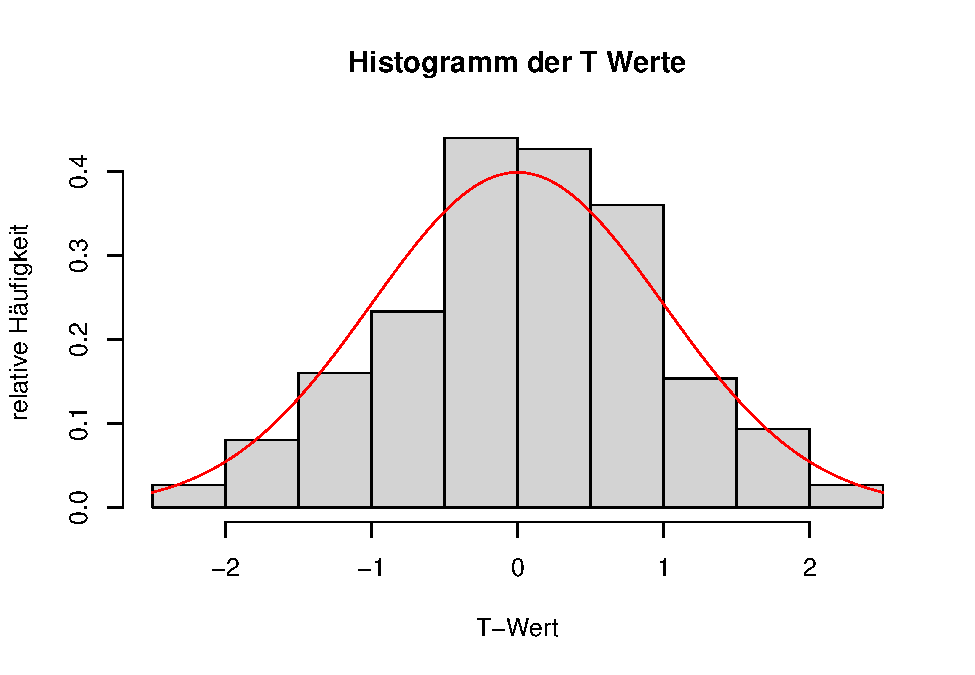
\includegraphics{Test_files/figure-latex/unnamed-chunk-5-1.pdf}

\begin{Shaded}
\begin{Highlighting}[]
\CommentTok{#Kolmogorov-Smirnoff-Test}
\KeywordTok{print}\NormalTok{(}\KeywordTok{ks.test}\NormalTok{(Tdata, }\StringTok{"pt"}\NormalTok{, }\KeywordTok{length}\NormalTok{(data)}\OperatorTok{-}\DecValTok{1}\NormalTok{))}
\end{Highlighting}
\end{Shaded}

\begin{verbatim}
## 
##  One-sample Kolmogorov-Smirnov test
## 
## data:  Tdata
## D = 0.068075, p-value = 0.124
## alternative hypothesis: two-sided
\end{verbatim}

Da der \(p\)-Wert des Kolmogorov-Smirnoff-Tests kleiner als \(1-\alpha=0.95\) ist, kann die Nullhypothese nicht verworfen werden,
also ist die Verteilung der Teststatistik t-verteilt.

QQ-Plot:

\begin{Shaded}
\begin{Highlighting}[]
\KeywordTok{qqnorm}\NormalTok{(Tdata)}
\KeywordTok{qqline}\NormalTok{(Tdata)}
\end{Highlighting}
\end{Shaded}

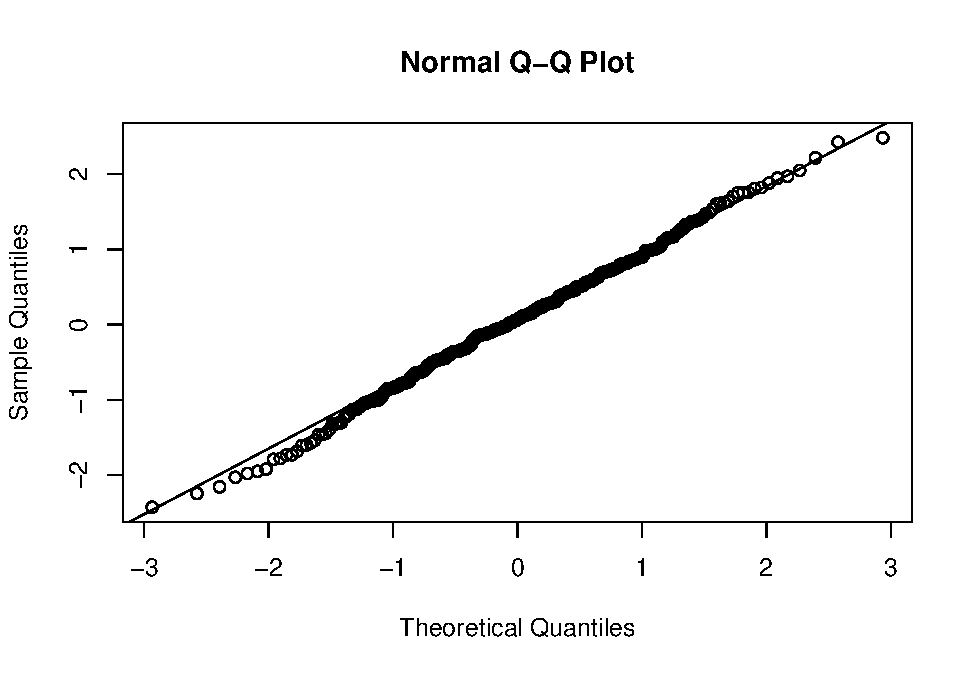
\includegraphics{Test_files/figure-latex/unnamed-chunk-6-1.pdf}
Ergebnis: Alles deutet darauf hin, dass die Teststatistik t-verteilt ist.

\hypertarget{t-test-mit-bekannter-varianz}{%
\subsection{\texorpdfstring{\(t-\)Test mit bekannter Varianz}{t-Test mit bekannter Varianz}}\label{t-test-mit-bekannter-varianz}}

Genau wie oben, nur dass wir die Varianz nicht schätzen müssen.
Deshalb ist die Teststatistik \(\sqrt{n}\dfrac{\bar X_n-\mu_0}{\sigma}\sim N(0,1)\).
Der Rest bleibt gleich:

\begin{Shaded}
\begin{Highlighting}[]
\KeywordTok{set.seed}\NormalTok{(}\DecValTok{123}\NormalTok{)}
\NormalTok{mu0 <-}\StringTok{ }\DecValTok{2}
\NormalTok{sigma <-}\StringTok{ }\DecValTok{4}
\NormalTok{data <-}\StringTok{ }\KeywordTok{rnorm}\NormalTok{(}\DecValTok{1000}\NormalTok{, mu0, sigma)}
\NormalTok{alpha <-}\StringTok{ }\FloatTok{0.05}

\NormalTok{dataMean <-}\StringTok{ }\KeywordTok{mean}\NormalTok{(data)}

\NormalTok{T <-}\StringTok{ }\KeywordTok{sqrt}\NormalTok{(}\KeywordTok{length}\NormalTok{(data))}\OperatorTok{*}\NormalTok{(dataMean}\OperatorTok{-}\NormalTok{mu0)}\OperatorTok{/}\NormalTok{sigma}

\CommentTok{#Teststatistik}
\KeywordTok{print}\NormalTok{(}\KeywordTok{paste}\NormalTok{(}\StringTok{"T = "}\NormalTok{, T))}
\end{Highlighting}
\end{Shaded}

\begin{verbatim}
## [1] "T =  0.51000790152087"
\end{verbatim}

\begin{Shaded}
\begin{Highlighting}[]
\CommentTok{#p-Wert von T unter Normalverteilung}
\KeywordTok{print}\NormalTok{(}\KeywordTok{paste}\NormalTok{(}\StringTok{"p-Wert von T = "}\NormalTok{, }\KeywordTok{pnorm}\NormalTok{(T, }\KeywordTok{length}\NormalTok{(data)}\OperatorTok{-}\DecValTok{1}\NormalTok{, }\DataTypeTok{lower.tail =} \OtherTok{FALSE}\NormalTok{)))}
\end{Highlighting}
\end{Shaded}

\begin{verbatim}
## [1] "p-Wert von T =  1"
\end{verbatim}

\begin{Shaded}
\begin{Highlighting}[]
\CommentTok{#Testresultat}
\ControlFlowTok{if}\NormalTok{ (}\KeywordTok{pnorm}\NormalTok{(T, }\DataTypeTok{lower.tail =} \OtherTok{FALSE}\NormalTok{) }\OperatorTok{>}\StringTok{ }\DecValTok{1}\OperatorTok{-}\NormalTok{alpha)\{}
  \KeywordTok{print}\NormalTok{(}\StringTok{"Nullhypothese wird verworfen"}\NormalTok{)}
\NormalTok{\} }\ControlFlowTok{else}\NormalTok{ \{}
  \KeywordTok{print}\NormalTok{(}\StringTok{"Nullhypothese wird nicht verworfen"}\NormalTok{)}
\NormalTok{\}}
\end{Highlighting}
\end{Shaded}

\begin{verbatim}
## [1] "Nullhypothese wird nicht verworfen"
\end{verbatim}

Verteilung der Teststatistik:

\begin{Shaded}
\begin{Highlighting}[]
\KeywordTok{set.seed}\NormalTok{(}\DecValTok{123}\NormalTok{)}
\NormalTok{Tdata =}\StringTok{ }\KeywordTok{c}\NormalTok{()}

\ControlFlowTok{for}\NormalTok{ (i }\ControlFlowTok{in} \DecValTok{1}\OperatorTok{:}\DecValTok{300}\NormalTok{)\{}
\NormalTok{  data <-}\StringTok{ }\KeywordTok{rnorm}\NormalTok{(}\DecValTok{1000}\NormalTok{, mu0, sigma)}
\NormalTok{  alpha <-}\StringTok{ }\FloatTok{0.05}

\NormalTok{  T <-}\StringTok{ }\KeywordTok{sqrt}\NormalTok{(}\KeywordTok{length}\NormalTok{(data))}\OperatorTok{*}\NormalTok{(}\KeywordTok{mean}\NormalTok{(data)}\OperatorTok{-}\NormalTok{mu0)}\OperatorTok{/}\NormalTok{sigma}
\NormalTok{  Tdata =}\StringTok{ }\KeywordTok{c}\NormalTok{(Tdata, T)}
\NormalTok{\}}
\KeywordTok{hist}\NormalTok{(Tdata, }\DataTypeTok{freq=}\OtherTok{FALSE}\NormalTok{, }\DataTypeTok{main =} \StringTok{"Histogramm der T Werte"}\NormalTok{, }\DataTypeTok{xlab =} \StringTok{"T-Wert"}\NormalTok{, }\DataTypeTok{ylab =} \StringTok{"relative Häufigkeit"}\NormalTok{)}
\KeywordTok{curve}\NormalTok{(}\KeywordTok{dnorm}\NormalTok{(x), }\DataTypeTok{add =} \OtherTok{TRUE}\NormalTok{, }\DataTypeTok{col =} \StringTok{"red"}\NormalTok{)}
\end{Highlighting}
\end{Shaded}

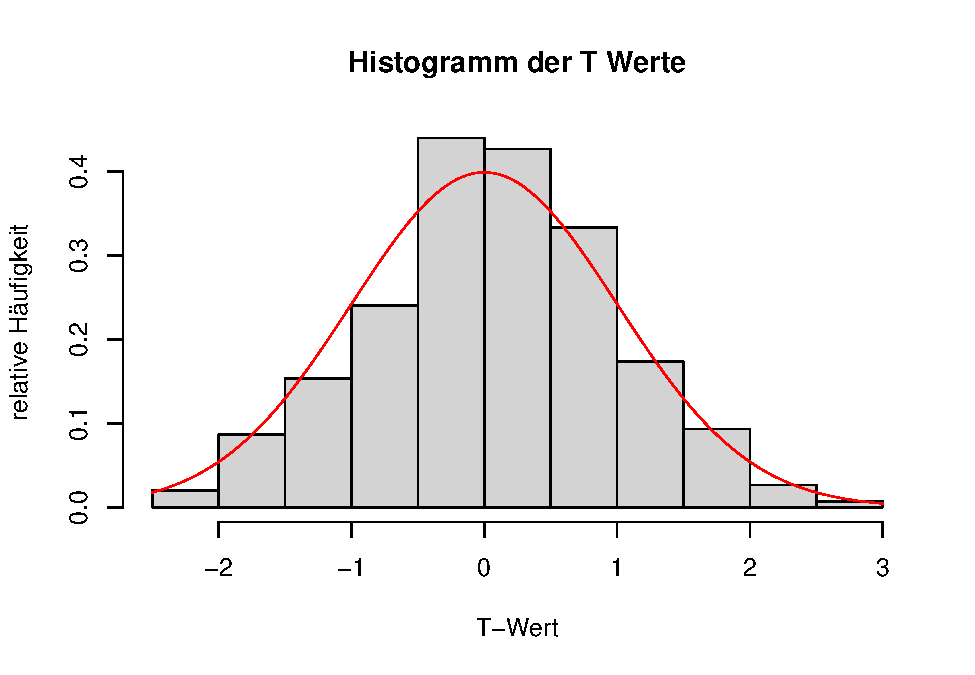
\includegraphics{Test_files/figure-latex/unnamed-chunk-8-1.pdf}

\begin{Shaded}
\begin{Highlighting}[]
\CommentTok{#Kolmogorov-Smirnoff-Test}
\KeywordTok{print}\NormalTok{(}\KeywordTok{ks.test}\NormalTok{(Tdata, }\StringTok{"pnorm"}\NormalTok{, }\DataTypeTok{lower.tail =} \OtherTok{FALSE}\NormalTok{))}
\end{Highlighting}
\end{Shaded}

\begin{verbatim}
## 
##  One-sample Kolmogorov-Smirnov test
## 
## data:  Tdata
## D = 0.99456, p-value < 2.2e-16
## alternative hypothesis: two-sided
\end{verbatim}

Da der \(p\)-Wert des Kolmogorov-Smirnoff-Tests kleiner als \(1-\alpha=0.95\) ist, kann die Nullhypothese nicht verworfen werden,
also ist die Verteilung der Teststatistik t-verteilt.

QQ-Plot:

\begin{Shaded}
\begin{Highlighting}[]
\KeywordTok{qqnorm}\NormalTok{(Tdata)}
\KeywordTok{qqline}\NormalTok{(Tdata)}
\end{Highlighting}
\end{Shaded}

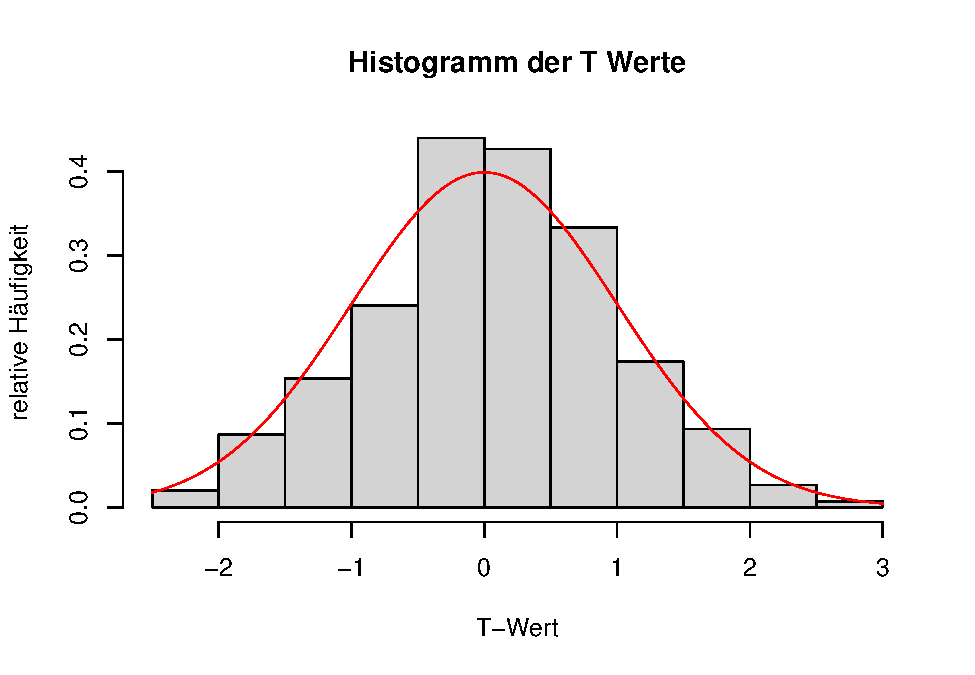
\includegraphics{Test_files/figure-latex/unnamed-chunk-9-1.pdf}
Ergebnis: Alles deutet darauf hin, dass die Teststatistik normalverteilt ist.

\hypertarget{aufgabe-2}{%
\section{Aufgabe 2}\label{aufgabe-2}}

Lineare Regression mit R

\hypertarget{daten-einlesen}{%
\subsection{Daten einlesen}\label{daten-einlesen}}

\begin{Shaded}
\begin{Highlighting}[]
\NormalTok{data <-}\StringTok{ }\KeywordTok{read.table}\NormalTok{(}\StringTok{"Datensaetze/wine.txt"}\NormalTok{, }\DataTypeTok{header =} \OtherTok{TRUE}\NormalTok{)}
\end{Highlighting}
\end{Shaded}

\hypertarget{uxfcberblick-uxfcber-die-daten}{%
\subsection{Überblick über die Daten}\label{uxfcberblick-uxfcber-die-daten}}

\begin{Shaded}
\begin{Highlighting}[]
\KeywordTok{head}\NormalTok{(data)}
\end{Highlighting}
\end{Shaded}

\begin{verbatim}
##   year price temp h.rain w.rain
## 1 1952    37 17.1    160    600
## 2 1953    63 16.7     80    690
## 3 1955    45 17.1    130    502
## 4 1957    22 16.1    110    420
## 5 1958    18 16.4    187    582
## 6 1959    66 17.5    187    485
\end{verbatim}

\begin{Shaded}
\begin{Highlighting}[]
\KeywordTok{summary}\NormalTok{(data)}
\end{Highlighting}
\end{Shaded}

\begin{verbatim}
##       year          price             temp           h.rain     
##  Min.   :1952   Min.   : 10.00   Min.   :15.00   Min.   : 38.0  
##  1st Qu.:1960   1st Qu.: 14.00   1st Qu.:16.15   1st Qu.: 88.0  
##  Median :1967   Median : 22.00   Median :16.40   Median :123.0  
##  Mean   :1967   Mean   : 28.81   Mean   :16.47   Mean   :144.8  
##  3rd Qu.:1974   3rd Qu.: 35.00   3rd Qu.:17.00   3rd Qu.:185.5  
##  Max.   :1980   Max.   :100.00   Max.   :17.60   Max.   :292.0  
##      w.rain     
##  Min.   :376.0  
##  1st Qu.:543.5  
##  Median :600.0  
##  Mean   :608.4  
##  3rd Qu.:705.5  
##  Max.   :830.0
\end{verbatim}

\hypertarget{lineares-modell}{%
\subsection{Lineares Modell}\label{lineares-modell}}

\begin{Shaded}
\begin{Highlighting}[]
\NormalTok{model <-}\StringTok{ }\KeywordTok{lm}\NormalTok{(price }\OperatorTok{~}\StringTok{ }\NormalTok{temp }\OperatorTok{+}\StringTok{ }\NormalTok{h.rain }\OperatorTok{+}\StringTok{ }\NormalTok{w.rain, }\DataTypeTok{data =}\NormalTok{ data)}
\KeywordTok{summary}\NormalTok{(model)}
\end{Highlighting}
\end{Shaded}

\begin{verbatim}
## 
## Call:
## lm(formula = price ~ temp + h.rain + w.rain, data = data)
## 
## Residuals:
##     Min      1Q  Median      3Q     Max 
## -16.580  -8.601  -4.057   6.813  29.064 
## 
## Coefficients:
##               Estimate Std. Error t value Pr(>|t|)    
## (Intercept) -365.45179   77.63849  -4.707 9.66e-05 ***
## temp          22.50086    4.28502   5.251 2.51e-05 ***
## h.rain        -0.09296    0.03746  -2.481   0.0208 *  
## w.rain         0.06103    0.02247   2.717   0.0123 *  
## ---
## Signif. codes:  0 '***' 0.001 '**' 0.01 '*' 0.05 '.' 0.1 ' ' 1
## 
## Residual standard error: 13.33 on 23 degrees of freedom
## Multiple R-squared:  0.6421, Adjusted R-squared:  0.5954 
## F-statistic: 13.75 on 3 and 23 DF,  p-value: 2.389e-05
\end{verbatim}

In dem linearen Modell hat der Temperaturkoeffzient ein positives Vorzeichen, was bedeutet,
dass der Preis mit steigender Temperatur steigt.\\
Der Koeffizient für Niederschlag bei der Ernte hat ein negatives Vorzeichen, was bedeutet,
dass der Preis mit steigendem Niederschlag bei der Ernte sinkt.
Der Koeffizient für Niederschlag im Winter hat ein positives Vorzeichen, was bedeutet,
dass der Preis mit steigendem Niederschlag im Winter steigt.

\end{document}
